\section{Modeling of Ablating Thermal Protection Systems}

This section presents the problem of modeling ablation for a non-decomposing TPS as a parametrized system of coupled non-linear PDEs. The ablation physics is decomposed into heat conduction and mesh motion, which are governed by the energy and pseudo-elasticity PDEs, respectively. Predictions for the ablating TPS response computed based on two models: (1) a high-fidelity FOM based on discontinuous Galerkin FEM (DG-FEM), and (2) an RPM based on the LCM. The mathematical details for the governing equations, FOM, and RPM, are provided next.

\subsection{Governing Equations}\label{sec_governing_equations}

\paragraph*{Heat Conduction} Consider a generic domain $\Omega\subset$, $d=2$ or $3$, illustrated in Fig.~\ref{fig_general_domain}. Let $\partial\Omega = \Gamma_q\cup\Gamma_T$ and $\Gamma_q\cap\Gamma_T = \emptyset$, where a Neumann $q_b(x,t)$ boundary condition is prescribed on the $\Gamma_q$ boundary, and a Dirichlet $T_b(x,t)$ boundary condition is prescribed on the boundary $\Gamma_T$. The ablation is modeled as mesh motion, and occurs only on the heated boundary $\Gamma_q$. Ablating effects on the energy equation are handled using the Arbitrary Lagrangian-Eulerian (ALE) description. The ALE establishes that mesh displacements $w(x,t)\in\mathbb{R}^d$ and velocities $v(x,t)\in\mathbb{R}^d$ evolve independently of the physical material's displacements, which are set to zero~\hl{CITE}.

\begin{figure}
    \centering
    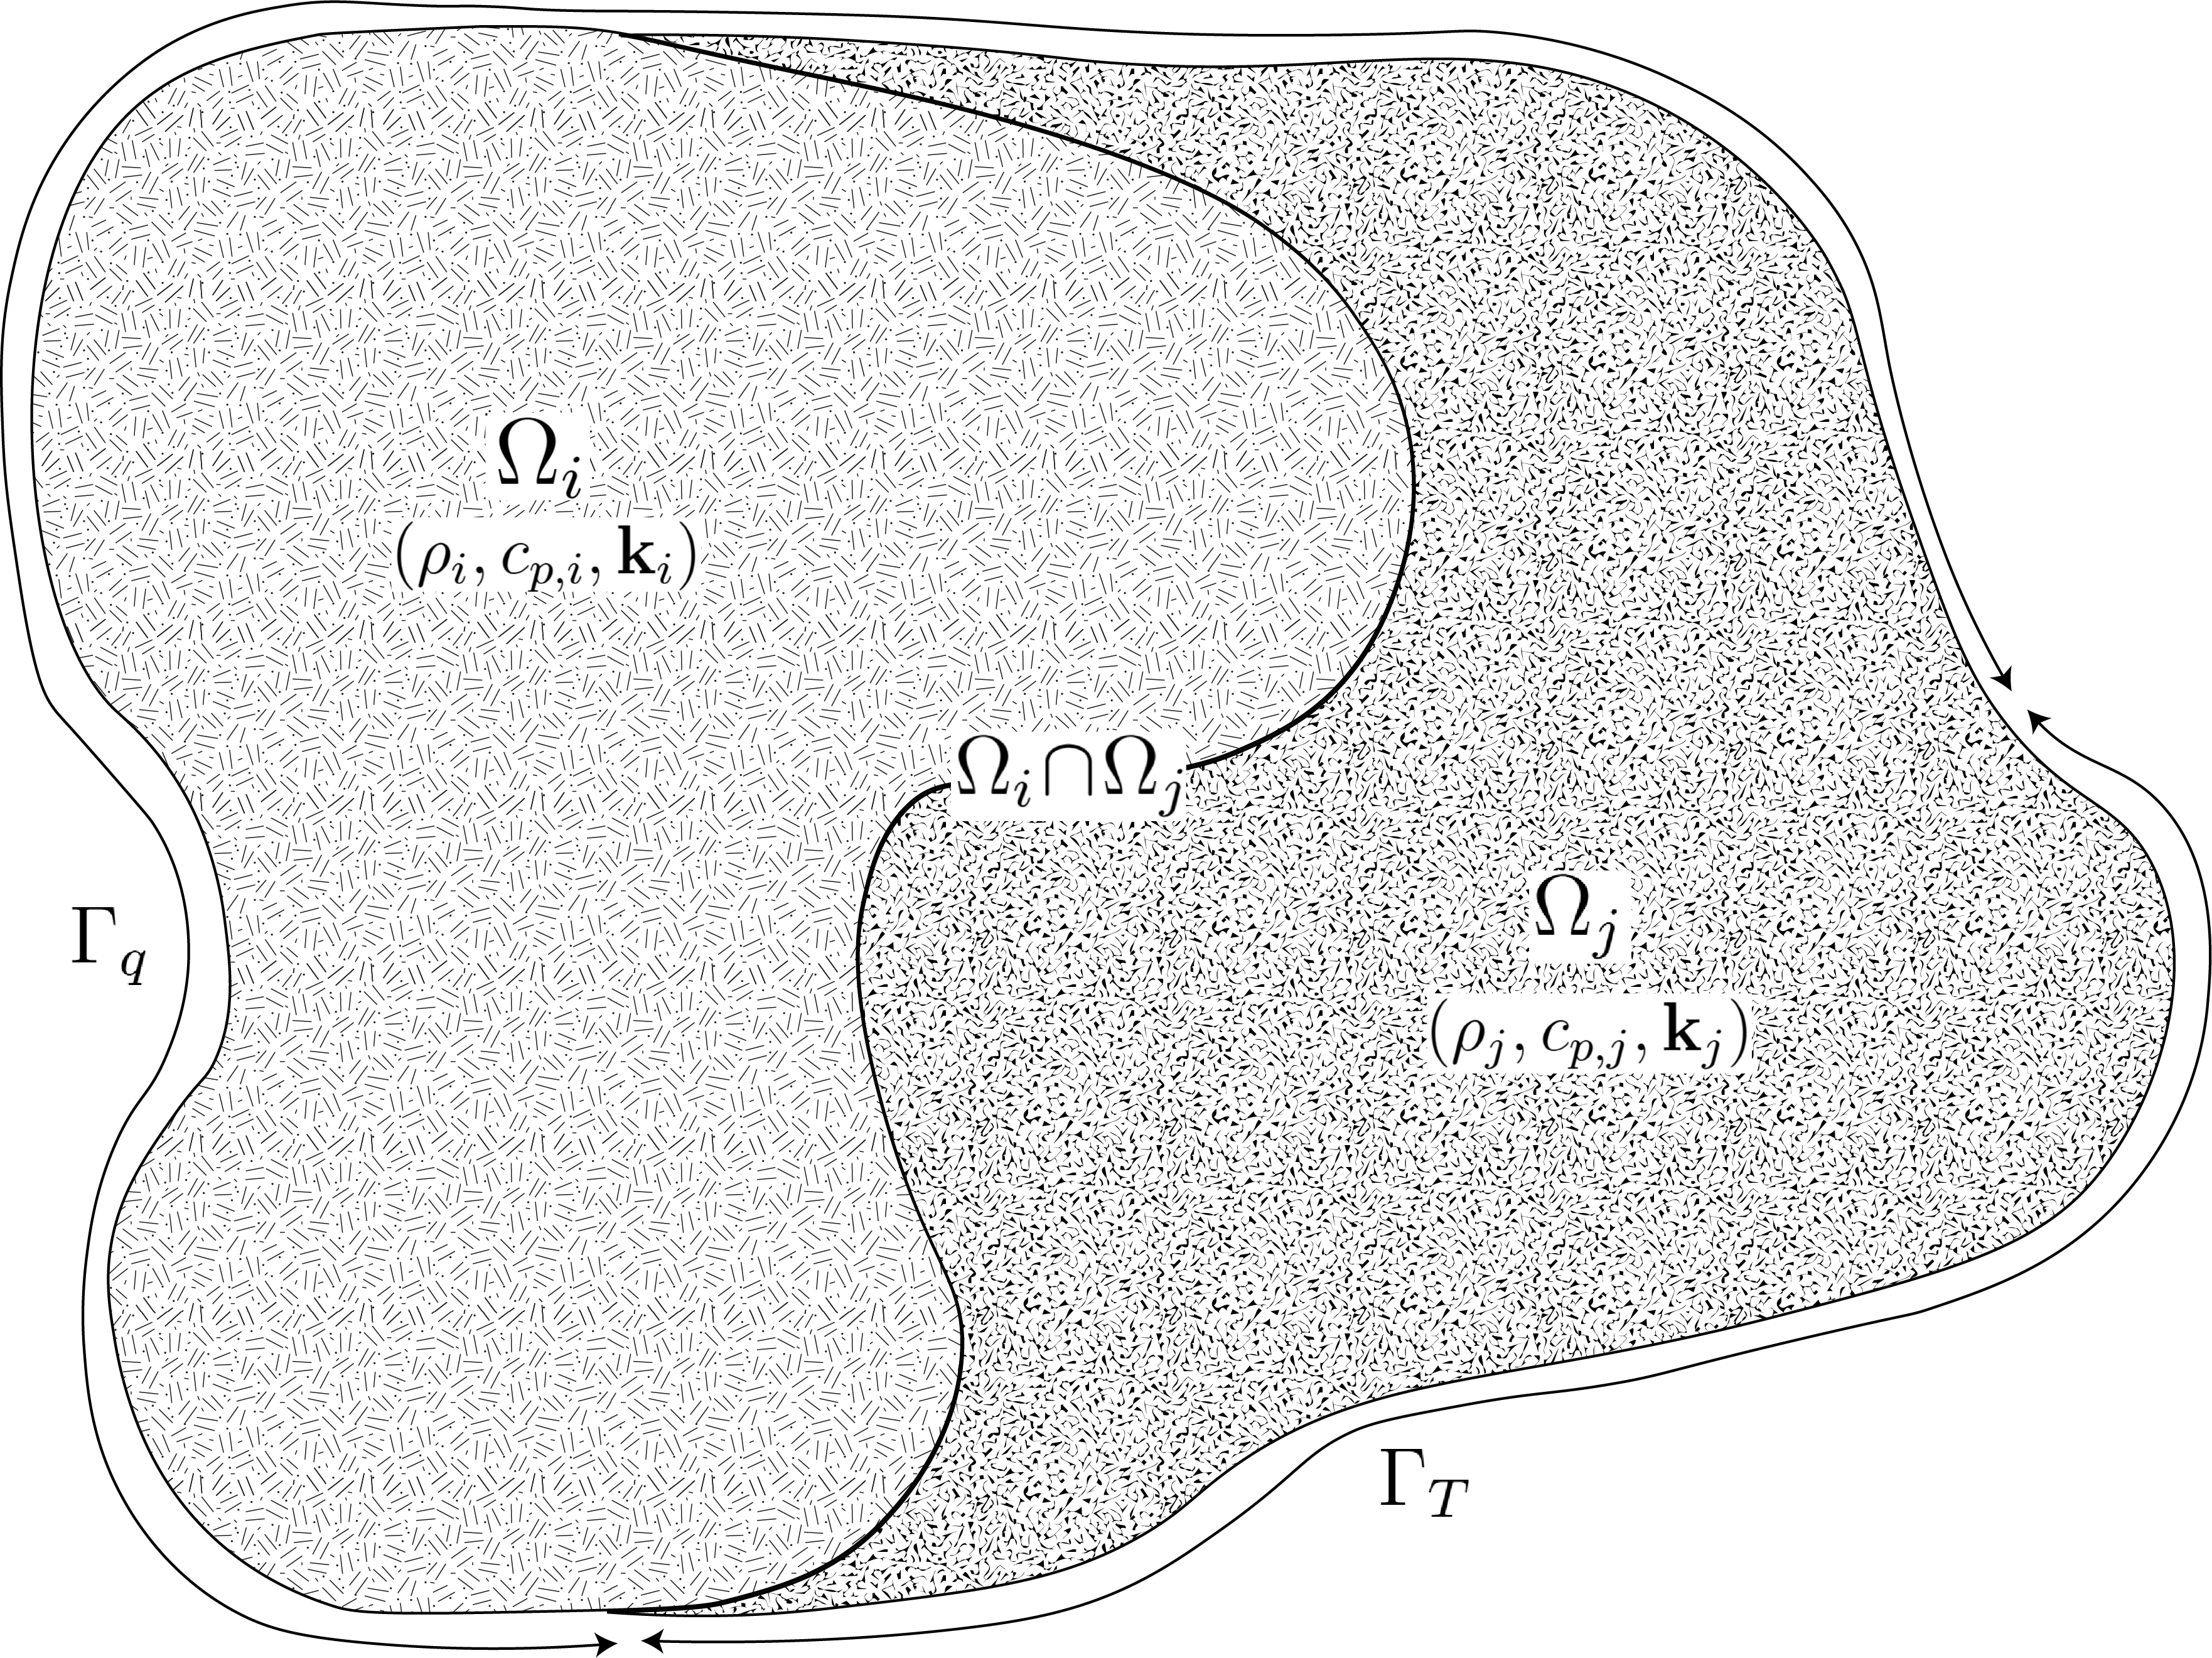
\includegraphics[width=0.6\textwidth]{./figs/general_domain.png}
    \caption{General domain $\Omega$ with prescribed Neumann and Dirichlet boundary conditions on $\Gamma_q$ and $\Gamma_T$. Mesh displacement $w(x,t)$ occurs on the $\Gamma_q$ boundary.}
    \label{fig_general_domain}
\end{figure}

The transient heat conduction is described by the energy equation,
\begin{subequations}
    \begin{align}
        \rho c_p\left(\ppt{T} - v(x,t)\cdot\nabla T\right) - \nabla\cdot (\mathbf{k}\nabla T) &= \cQ(x,t),\ x\in\Omega \label{eqn_thermal_pde}\\
        -\mathbf{k}\nabla T\cdot \vn &= q_b(x,t),\ x\in\Gamma_q\label{eqn_thermal_bc_neumann}\\
        T(x,t) &= T_b(x,t),\ x\in\Gamma_T\label{eqn_thermal_bc_dirichlet}\\
        T(x,0) &= T_0(x),\ x\in\Omega\label{eqn_thermal_ic}
    \end{align}\label{eqn_governing_equations}
\end{subequations}
where the density $\rho$ is constant, while the heat capacity $c_p$ and thermal conductivity $\mathbf{k}\in\mathbb{R}^{d\times d}$, are temperature dependent. In the order they appear, the terms in \cref{eqn_thermal_pde} include, the unsteady energy storage, heat conduction, temperature advection due to mesh motion, and source terms due to boundary conditions.

\paragraph*{Mesh Motion} The mesh motion is described by the pseudo-elasticity equation,
\begin{subequations}
    \begin{align}
        \nabla\cdot\sigma(w) &= 0\label{eqn_elasticity_pde}\\
        w(x,t) &= w_q(x,t),\quad x\in\Gamma_q\label{eqn_displacement_heated_bc}\\
        w(x,t) &= 0,\quad x\notin \Gamma_q\label{eqn_displacement_unheated_bc}\\
        w(x,0) &= \boldsymbol{0}\label{eqn_displacement_initial_condition}
    \end{align}
\end{subequations}
where the stress tensor $\sigma$ is related to the strain tensor $\bepsilon(w)$ through Hooke's law,
\[
    \sigma(w) = \mathbb{D}:\boldsymbol{\epsilon}(w)
\]
where $\mathbb{D}$ is the constitutive operator, ``:'' is the double contraction of tensors, and $\bepsilon$ is the symmetric strain tensor given by,
\[
    \bepsilon(\bw) = \frac{1}{2}\left(\nabla\bw + \nabla\bw^T\right)
\]
For instance, an isotropic material assumption results in,
\[
    \bsigma = \lambda\left(\nabla\cdot\bw\right) \mathbf{I} + 2\mu\bepsilon(\bw)
\]
where $\lambda$ and $\mu$ are Lame constants that are arbitrarily selected to model the mesh motion. The ``material'' properties $\lambda$ and $\mu$ can be chosen to tailor the mesh deformation and need not represent the actual material being modeled~\hl{Amar2016}. 

The boundary conditions for the energy equation includes a heated surface (\cref{eqn_thermal_bc_neumann}) and a constant-temperature surface (\cref{eqn_thermal_bc_dirichlet}). The boundary conditions for the pseudo-elasticity equation are a function of the surface temperature $T_q(x,t)$ for $x\in\Gamma_q$ using a B' table. The B' table....
\begin{equation}
    \bw_q(x,t) = \int_{0}^{t} \mathbf{v}(x,\tau)d\tau = \int_{0}^{t}\mathbf{f}\left(T_q(x,\tau)\right)d\tau\label{eqn_boundary_displacement}
\end{equation}

\subsection{Full-Order Model: Finite-Element Method}\label{sec_fom}

To obtain the full-order numerical solution, the governing equation is spatially discretized using variational principles of Discontinuous Galerkin (DG) to result in a high-dimensional system of ordinary differential equations (ODEs). Note that the choice of DG approach here is mainly for theoretical convenience in the coarse-graining formulation, and is exclusively performed on the energy equation as the quantities of interest correspond to the ablating surface temperatures. In Sec.~\hl{x}, the high-fidelity ablating TPS solution is performed using standard FEM for both the energy and elastictiy equations, and the equivalence between DG and standard FEM is noted upon their convergence.

Consider a conforming mesh partition domain, where each element belongs to one and only one component. Denote the collection of all $M$ elements as $\left\{E_i\right\}_{i=1}^{M}$. In an element $E_i$, its shared boundaries with another element $E_j$, Neumann BC, and Dirichlet BC are denoted as $e_{ij}$, $e_{iq}$, and $e_{iT}$, respectively. Lastly, $\left|e\right|$ denotes the length $(n_d=2)$ or area $(n_d=3)$ of a component boundary $e$.

For the $i$-th element, use a set of $P$ trial functions, such as polynomials, to represent the temperature distribution,
\begin{equation}
    T^{(i)}(x,t) = \sum_{l=1}^{P} \phi_l^{(i)}(x)u_l^{(i)} \equiv \boldsymbol{\phi}^{(i)}(x)^T\vu^{(i)}(t),\quad i=1,2,\dots,M\label{eqn_element_temperature}
\end{equation}
By standard variational processes, e.g., \hl{Cohen2018}, the element-wise governing equation is denoted as,
\begin{equation}
    \vA^{(i)}\dot{\vu}^{(i)} = \left(\vB^{(i)} + \vC^{(i)}(t)\right)\vui + \sumneighbordirichlet\left(\vB^{(i)}_{ij}\vui + \vB^{(j)}_{ij}\vuj\right) + \vf^{(i)}(t),\quad\text{for }i=1,2,\dots,M\label{eqn_element_dg}
\end{equation}
which is collected as the following ODE for the all the elements in the mesh,
\begin{equation}
    \vA(\vu)\dot{\vu} = \left[\vB(\vu) + \vC(t,\vu)\right]\vu + \mathbf{f}(t)\label{eqn_full_dg}
\end{equation}
where $\vu = \left[\vu^{(1)}, \vu^{(2)}, \ldots, \vu^{(M)}\right]^T\in\mathbb{R}^{MP}$ includes all the DG variables, $\mathbf{f}\in\mathbb{R}^{MP}$ is the external forcing, and the system matrices $\vA$, $\vB$, and $\vC$ are the matrices due to heat capacity, heat conduction, and temperature advection due to mesh motion, respectively. A detailed derivation of \cref{eqn_element_dg,eqn_full_dg} and their matrices is provided in Appendix~\cite{appendix}.

\subsection{Reduced-Physics Model}
The RPM for predicting the response of the ablating TPS consists of two components: (1) the LCM, and (2) tabulated data for ablating velocity as a function of surface temperature. The LCM is described as a first-order system of ODEs for predicting the average temperatures inside the ablating TPS, and provides a low-fidelity under-estimation for the ablating surface temperature. The temperature prediction from LCM is used in a B' table to determine the surface recession velocity, from which the displacements are obtained through integration.

\subsubsection{Lumped Capacitance Model}
The main results regarding the LCM are provided in this section; details of the implementation for the TPS in Fig.~\ref{fig_four_components} are provided in Appendix~\ref{appendix}. The LCM is a classical physics-based low-order model for predicting the temporal variation of average temperature in multiple interconnected components\hl{INCROPERA}. The LCM is derived at the component level from a point of view of energy conservation, and leads to the following system of ODEs for the average temperatures on the components,
\begin{equation}
    \bar{\vA}\dot{\bar{\vu}} = \bar{\vB}\left(\bar{\vu}\right)\bar{\vu} + \bar{\vf}(t)\label{eqn_lcm}
\end{equation}
where,
\begin{subequations}
    \begin{align}
       \bar{\vu} &= \left[\bar{u}^{(1)},\bar{u}^{(2)},\dots,\bar{u}^{(N)}\right]^T\in\mathbb{R}^{N}\\
        \bar{\vf} &= \left[\bar{f}^{(1)},\bar{f}^{(2)},\dots,\bar{f}^{(N)}\right]^T\in\mathbb{R}^{N}
    \end{align}
\end{subequations}
includes the average temperatures $\bar{\vu}$ and forcing inputs $\bar{\vf}$ for the $N$ components. For $i,j=1,2,\dots,N$ the $(i,j)$-th elements of the $\bar{\vA}\in\mathbb{R}^{N\times N}$, $\bar{\vB}\in\mathbb{R}^{N\times N}$, and $\bar{\vf}\in\mathbb{R}^{N}$ matrices are given by,
\begin{subequations}
    \begin{gather}
        \bar{A}^{(i)} = \begin{cases}
                \int_{\Omega^{(i)}}\rho c_p d\Omega^{(i)}, & i=j\\
                0, & i\neq j
            \end{cases},\quad \bar{B}_{ij} = \begin{cases}
            \sumneighbordirichlet\bar{B}^{(i)}_{ij}, &i=j \\
            \bar{B}^{(j)}_{ij}, & i\neq j
        \end{cases},\\ \bf^{(i)} = \begin{cases}
            |\eiq|\bar{q}^{(i)} + \frac{|\eiT|}{R_{i}}\bar{T}^{(i)}, & i=j \\ 
            0, & i\neq j
        \end{cases}
    \end{gather}\label{eqn_lcm_matrices}
\end{subequations}
where,
\begin{equation}
    \bar{q}^{(i)} = \frac{1}{|\eiq|}\int_{\eiq} q_b d\eiq,\quad \bar{T}^{(i)} = \frac{1}{|\eiT|}\int_{\eiT}T_b d\eiT,\quad \bar{B}^{(i)}_{ij} = -\frac{|\eij|}{R_{ij}},\quad \bar{B}_{ij}^{(j)} = \frac{|\eij|}{R_{ij}}\label{eqn_lcm_matrices_elements}
\end{equation}

\begin{figure}
    \centering
    \subfigure[TPS Decomposition]{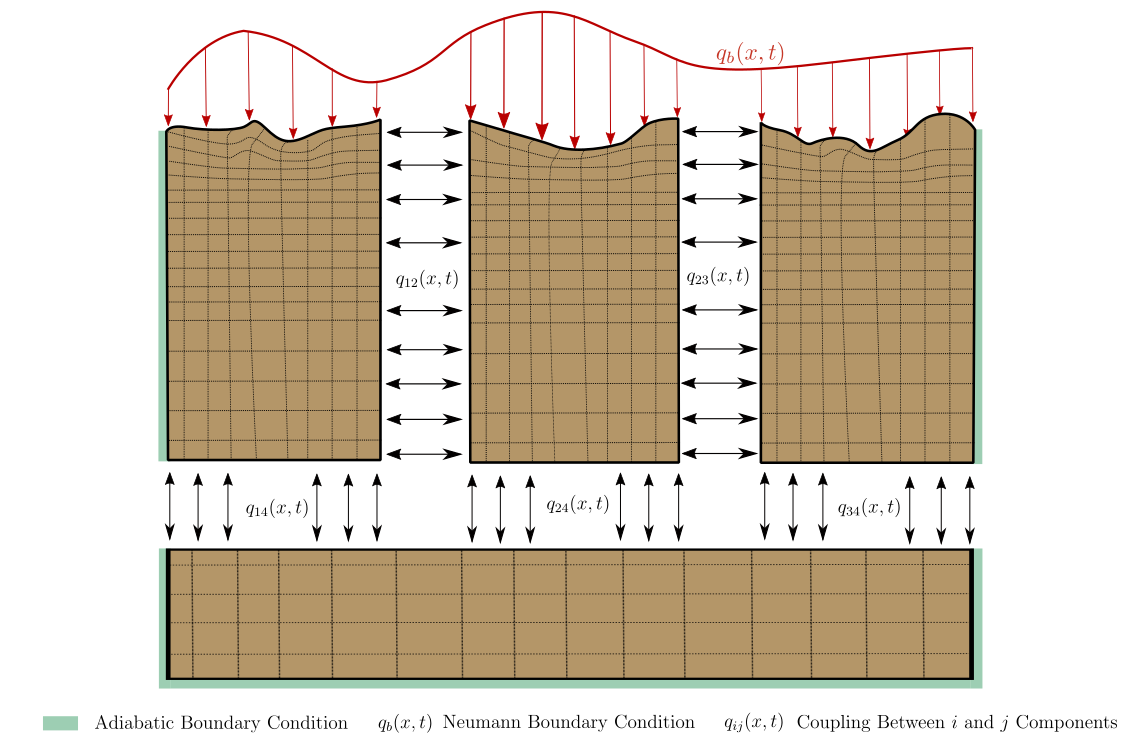
\includegraphics[width=0.8\textwidth]{./figs/four_components.png}}
    \subfigure[Lumped Mass Representation]{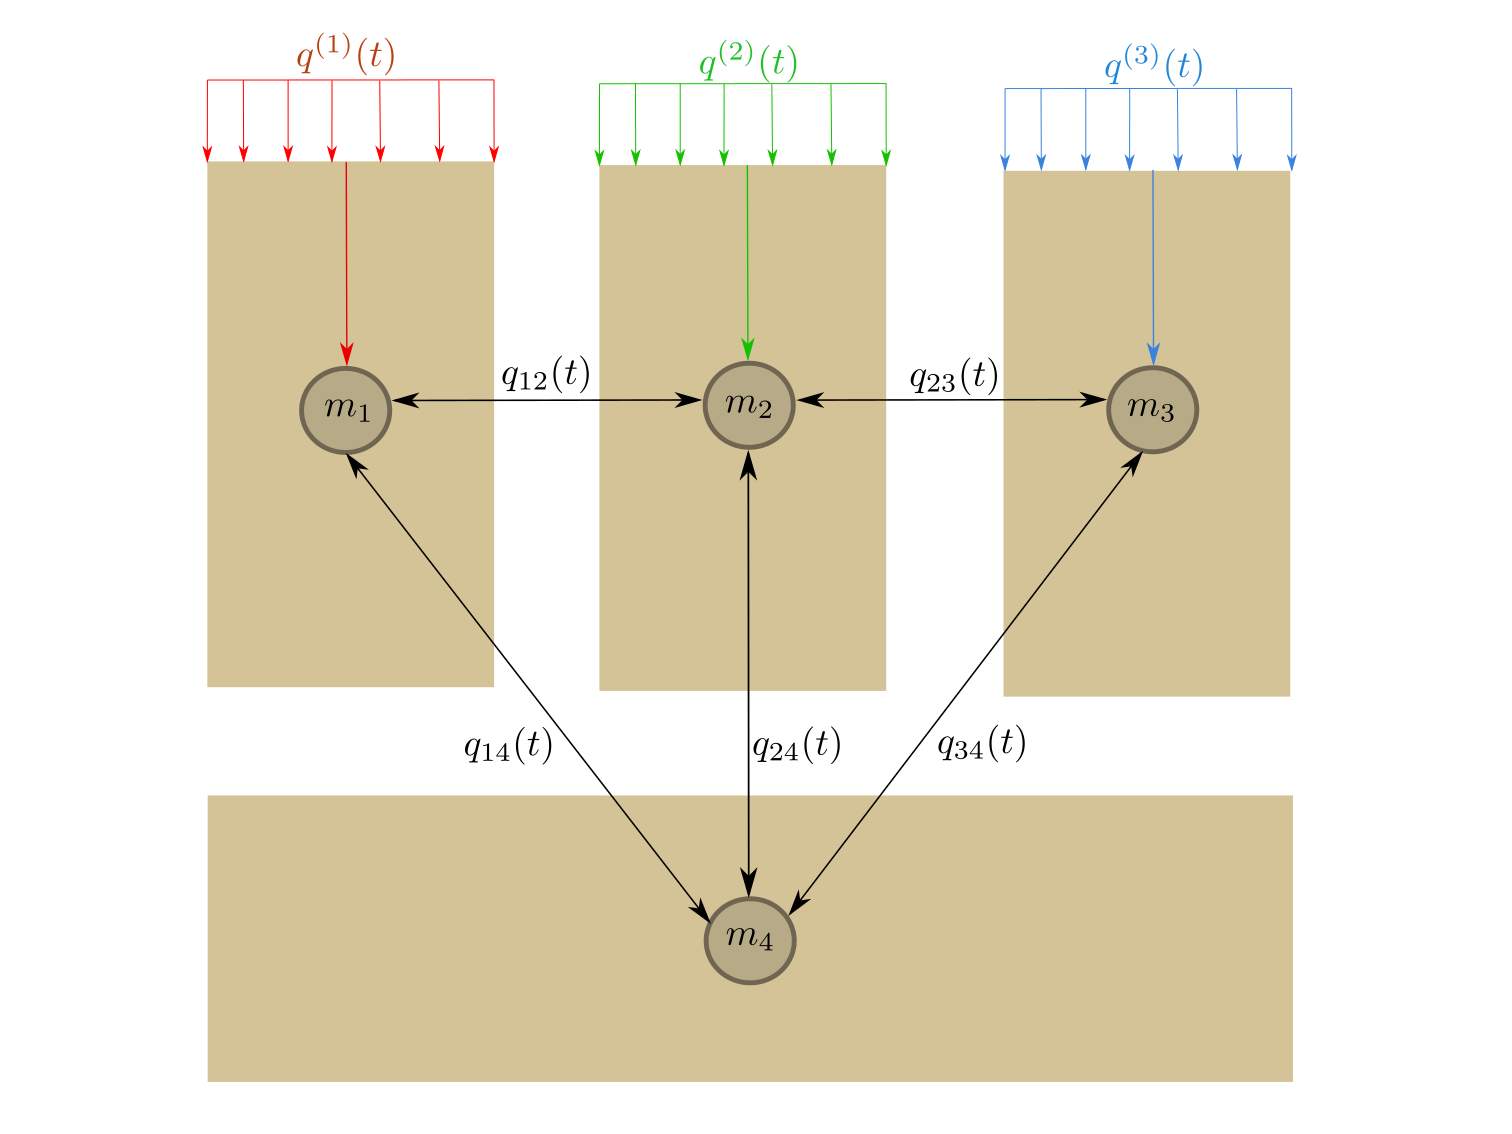
\includegraphics[width=0.8\textwidth]{./figs/lumped_mass_representation.png}}
    \caption{Partition of the TPS into three ablating and one non-ablating components with the corresponding lumped-mass representation.}
    \label{fig_four_components}
\end{figure}

\subsubsection{Surface Recession Velocity and Displacements}
Surface displacements are assumed to be one-dimensional and parallel to the surface normal $\vn$ of the heated boundary $\Gamma_q$. Thus, based on the $i$-th average temperature $\bu^{(i)}$ from LCM, the surface recession velocity and displacements are computed as,
\begin{equation}
    \dot{w}^{(i)}(t) = h^{(i)}(\bu^{(i)}),\quad w^{(i)}(t) = w^{(i)}(t_0) + \int_{t_0}^{t} h^{(i)}\left(\bu^{(i)}\right)d\tau
\end{equation}
where $h^{(i)}$ is a \hl{x} fit to the B' tabulated data for the material. \hl{Discussion of the B' tabulated data}. The B' table is pre-computed based on high-fidelity simulations of the ablation process for a one-dimensional slab of the material, and is independent of the TPS geometry and boundary conditions.

\subsection{Summary of Modeling Approaches}

The FOM (i.e., DG-FEM) and RPM (i.e., LCM) are two different but mathematically connected solution strategies. Specifically, the LCM in \cref{eqn_lcm} not only resembles the functional form of the DG model in \cref{eqn_full_dg}, but can be viewed as a special case of the latter, where the mesh partition is extremely coarse, and the trial and test functions are piece-wise constants. For example, consider the case where each component $\Omega^{(i)}$ is treated as one single element, and each element employs one constant basis function $\phi^{(i)}=1$. The element-wise DG model in \cref{eqn_element_dg} simplifies into a scalar ODE that ignores advection effects due to mesh motion,
\begin{equation}
    \vAi = \bar{A}^{(i)},\quad \vCi = 0, \quad\vBiij = -\sigma|\eij|,\quad \vBjij=\sigma|\eij|,\quad \vf^{(i)} = |\eiq|\bar{q}^{(i)} + \sigma|\eiT|\bar{T}^{(i)}
\end{equation}
Clearly, the LCM is a coarse zeroth-order DG model with the inverse of thermal resistance chosen as the element-wise penalty factors. Or conversely, the DG model is a refined version of LCM via \textit{hp}-adaptation.

The FOM and RPM represent two extremes in the modeling fidelity and computational cost spectrum. On one hand, the FOM is the most accurate but computationally expensive to evaluate due to the fine mesh discretizations for both the temperature and displacement fields, leading to possibly millions of state variables. On the other hand, the RPM considers only the average temperature of the material as the state variable, considerably reducing the computational cost, but sacrificing local temperature information and thus neglecting higher-order effects due to mesh motion. Thus, neither the FOM nor the RPM is a universal approach for real-world analysis, design, and optimization tasks for ablating TPS, where thousands of high-fidelity model evaluations may be necessary. This issue motivates the development of the PIROM, which can achieve the fidelity of FOM at a computational cost close to the RPM, while maintaining the generalizability to model parameters.